\documentclass{article}
\usepackage[spanish]{babel}
\usepackage[utf8]{inputenc}
\usepackage{graphicx}
\usepackage{minted}
\usepackage{courier}
\usepackage[dvipsnames]{xcolor}

\definecolor{pinkBlock}{rgb}{0.858, 0.188, 0.478}
\definecolor{greenBlock}{rgb}{0.109, 0.978, 0.244}

\title{\textbf{Criptografía aplicada: Cálculo del hash SHA-256 de un bloque Bitcoin}}
\author{Javier Domínguez Gómez \\
\small{jdg@member.fsf.org} \\
\small{Fingerprint: 94AD 19F4 9005 EEB2 3384 C20F 5BDC C668 D664 8E2B}}
\date{v0.1.03 - Febrero 2019}

\begin{document}
\maketitle

\tableofcontents{}

\section{Introducción}
    Este documento describe en detalle las partes de la cabecera de un bloque cualquiera en la cadena de bloques de Bitcoin, así como las operaciones lógico-matemáticas de la función criptográfica SHA-256 que se emplean con el fin de generar el \textit{hash} adecuado que finalmente representará dicho bloque en la cadena de bloques.

\section{Estructura de datos de un bloque}
    \vspace{3mm}
    Cada bloque de la cadena de bloques de Bitcoin contiene una estructura de datos que se puede categorizar en la siguiente tabla.
    \begin{table}[H]
    \centering
    \begin{tabular}{| c | l | c | l |} 
        \hline
        Tipo de dato & Nombre & Tamaño & Formato \\
        \hline
        uint32\_t & magicID & 4 bytes & Little-endian \\
        \hline
        uint32\_t & headerLenght & 4 bytes & Big-endian \\
        \hline
        uint32\_t & versionNumber & 4 bytes & Little-endian \\
        \hline
        uint8\_t[32] & previousBlockHash & 32 bytes & Big-endian \\
        \hline
        uint8\_t[32] & merkleRoot & 32 bytes & Big-endian \\
        \hline
        uint32\_t & timeStamp & 4 bytes & Little-endian \\
        \hline
        uint32\_t & targetDifficulty & 4 bytes & Little-endian \\
        \hline
        uint32\_t & nonce & 4 bytes & Little-endian \\
        \hline
        uint8/16/32/64\_t & transactionCount & 1, 3, 5 o 9 bytes & Big-endian*  \\
        \hline
    \end{tabular}
    \caption{Datos de la cabecera de un bloque en la cadena de bloques de Bitcoin.}
    \label{table:0}
    \end{table}
    
    *En el caso de \textit{transactionCount}, los enteros grandes se codifican en formato \textit{Little-endian}.
    
    \subsection{magicID}
    Se trata de un dato de 4 bytes de longitud. Se establece como prefijo en cada uno de los mensajes entre los nodos para identificar la red de Bitcoin en la que se generan. La siguiente tabla muestra los diferentes valores que puede tener la variable magicID dependiendo de la red.
    
    \begin{table}[H]
    \centering
    \begin{tabular}{| c | c |} 
        \hline
        Red & magicID \\
        \hline
        Mainnet & \texttt{0xf9beb4d9} \\
        \hline
        Testnet & \texttt{0xfabfb5da} \\
        \hline
        Testnet3 & \texttt{0x0b110907} \\
        \hline
        Namecoin & \texttt{0xf9beb4fe} \\
        \hline
        Regtest & \texttt{0xfabfb5da} \\
        \hline
    \end{tabular}
    \label{table:1}
    \end{table}
    
    No solo sirve como dato identificativo de una red en particular, también cumple la función de delimitador entre mensajes y entre los datos de cada bloque, pues estos vienen concatenados en cadenas hexadecimales uno a continuación de otro.
    
    Se decidió establecer estos valores tan específicos dada la improbabilidad de que los caracteres ASCII que representan se encuentren en un mensaje estándar, tal y como se indica en el archivo \textit{chainparams.cpp}\footnote{https://github.com/bitcoin/bitcoin/blob/master/src/chainparams.cpp\#L99} que lo implementa en el código de Bitcoin.
    
    \subsection{headerLenght}
    Este dato representa la longitud en bytes del bloque actual.
    
    \subsection{versionNumber}
    Este dato puede cambiar de valor cuando se actualiza el software y cambia el número de la versión del protocolo. El valor actual es 0x02000000 y se codifica en formato \textit{Little-endian}.
    
    \subsection{previousBlockHash}
    Se trata del \textit{hash} o \textit{digest} resultante del bloque anterior tras aplicar las funciones criptográficas utilizando los datos de la cabecera de dicho bloque. Tiene una longitud de 256 bits o 32 bytes codificado en formato \textit{Big-endian}.
    
    \subsection{merkleRoot}
    Este dato se modifica cada vez que una nueva transacción es aceptada. Tiene una longitud de 256 bits o 32 bytes codificado en formato \textit{Big-endian}
    
    \begin{figure}[H]
    \centering
        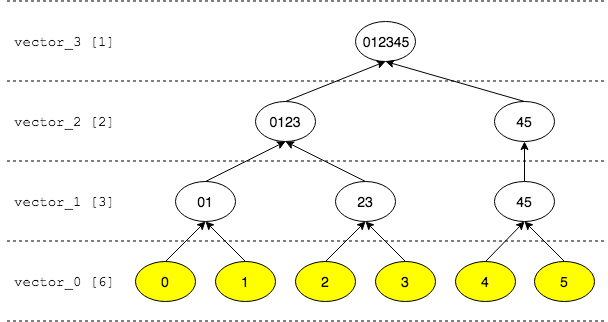
\includegraphics[scale=0.55]{img/Merkle_tree_05_leaves_nodes}
        \caption{Ejemplo de árbol de Merkle con 5 nodos hoja}
    \end{figure}
    
    \subsection{timeStamp}
    Se trata de un dato de 4 bytes de longitud en un formato numérico llamado Epoch o Tiempo Unix. Representa el número de segundos que han transcurrido desde el 1 de enero de 1970 a las 00:00. Se codifica en formato \textit{Little-endian}.
    
    Un ejemplo de cómo se puede calcular este dato es mediante el siguiente código C. Nótese que las horas se procesan como \textit{GMT+1}.
    \begin{figure}[H]
    \centering
        \begin{minted}{c}
    #include <stdio.h>
    #include <time.h>
    
    int main(int argc, char *argv[]) {
    
    	int year, month, day, hour, minute, second;
    	struct tm t;
    	time_t tod;
    
    	printf("Year: ");
    	scanf("%d", &year);
    	printf("Month: ");
    	scanf("%d", &month);
    	printf("Day: ");
    	scanf("%d", &day);
    	printf("Hour: ");
    	scanf("%d", &hour);
    	printf("Minute: ");
    	scanf("%d", &minute);
    	printf("Second: ");
    	scanf("%d", &second);
    
    	t.tm_year = year - 1900;
    	t.tm_mon = month - 1;   // Values [0-11]
    	t.tm_mday = day;
    	t.tm_hour = hour + 1;   // GMT+1
    	t.tm_min = minute;
    	t.tm_sec = second;
    	t.tm_isdst = 0;         // DST = 0
    	tod = mktime(&t);
    
    	printf("Timestamp epoch: %ld\n", (long) tod);
    }
        \end{minted}
    \end{figure}

    \subsection{targetDifficulty}
    Se trata de un número de 256 bits representado como un número decimal muy grande, tanto que abarcaría el rango de números que existen entre $0$ y $2^{256}-1$. Su función es la de definir una variable más a tener en cuenta a la hora de obtener el hash adecuado de un bloque antes de ser minado. Así pues la prueba de trabajo o \textit{Proof of Work} tendrá mayor o menor dificultad. En el protocolo de Bitcoin se define una regla que dice que el \textit{hash} del bloque ha de ser un número menor o igual al valor de la variable \textit{targetDifficulty} en ese momento. Así pues, si el \textit{hash} obtenido como candidato a generar un bloque fuera un número menor o igual al de \textit{targetDifficulty} habría posibilidades para que el \textit{hash} candidato sea un \textit{hash} válido para generar un nuevo bloque, aunque de forma adicional se han de cumplir otras condiciones. Por el contrario, si el \textit{hash} obtenido como candidato fuera un número mayor que el valor de la variable \textit{targetDifficulty}, se ha de incrementar el valor de la variable \textit{nonce} y probar otra vez a generar un \textit{hash} nuevo.
    
    \begin{figure}[H]
    \centering
        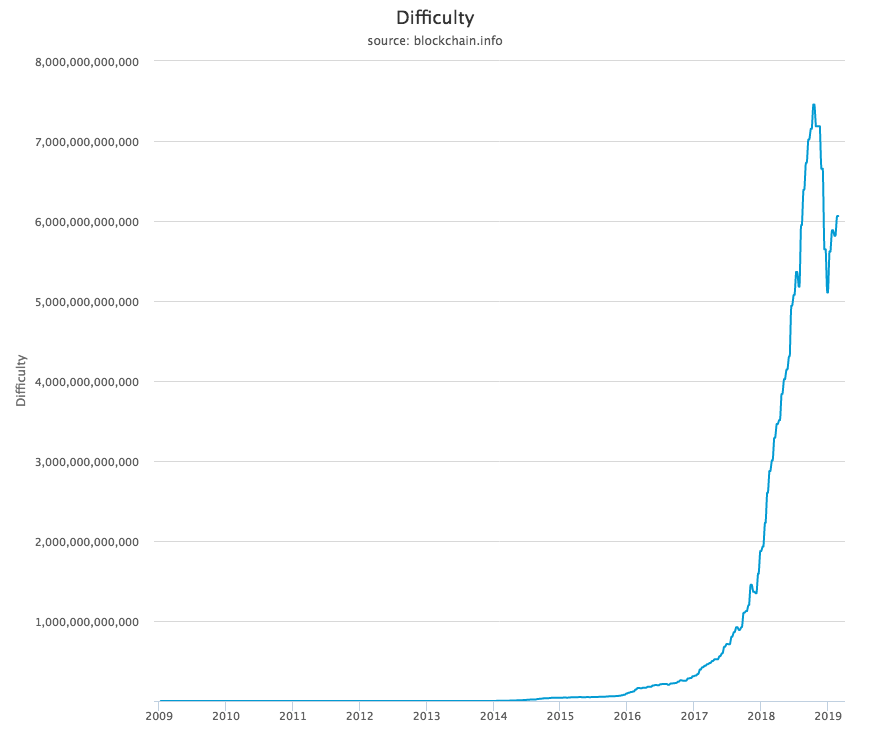
\includegraphics[scale=0.39]{img/Bitcoin_TargetDifficulty.png}
        \caption{Valor de la variable \textit{targetDifficulty} desde enero de 2009 hasta hoy.}
    \end{figure}
    
    El valor de la variable \textit{targetDifficulty} se modifica automáticamente una vez se han generado 2016 bloques, esto sucede aproximadamente cada dos semanas. El nuevo valor se obtiene mediante un cálculo que realizan todos los clientes Bitcoin de la red en el que toman el tiempo real que ha llevado generar los 2016 bloques y se obtiene la diferencia porcentual respecto al número de bloques que se esperaba haber calculado en el periodo de dos semanas.
    
    \subsection{nonce}
    Se trata de un número aleatorio con una longitud de 32 bits o 4 bytes codificado en formato \textit{Little-endian}.
    
    \subsection{transactionCount}
    En el caso de transactionCount el tipo de dato es un \textit{entero de longitud variable}\footnote{https://en.bitcoin.it/wiki/Protocol\_documentation\#Variable\_length\_integer}. Como el propio nombre indica, dependiendo de el número de transacciones que han sido procesadas tendrá un valor numérico u otro.
    
    \begin{figure}[H]
    \centering
        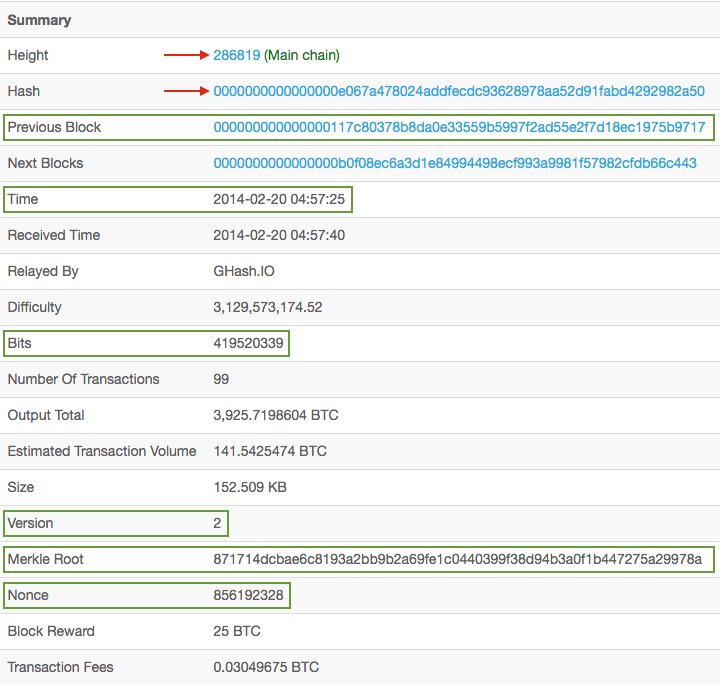
\includegraphics[scale=0.47]{img/Bitcoin_block_SHA_256_Block_Data}
        \caption{Datos empleados para la obtención del \textit{hash} del bloque $286819$.}
    \end{figure}
    
    \vspace{3mm}
    En la siguiente figura se detalla el contenido de los primeros 16 registros de la variable $W_{t}$ en cada una de las tres veces que se ejecutan las 64 iteraciones de la función SHA-256 para obtener el \textit{digest} en cada caso.
    \begin{figure}[H]
    \centering
        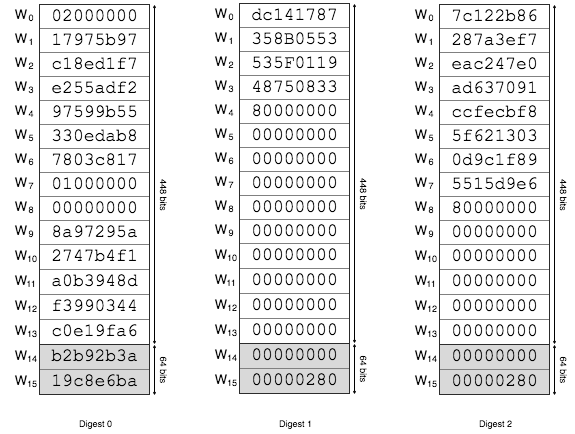
\includegraphics[scale=0.59]{img/Bitcoin_block_SHA_256_W0_W15_x3}
        \caption{Los primeros 16 registros de la variable $W_{t}$ en los tres casos en los que se ha de ejecutar la función SHA-256.}
    \end{figure}

\section{Almacenamiento en ficheros}
    A continuación un ejemplo de los datos de un bloque almacenados en un fichero blk*.dat.
    
    \begin{figure}[H]
    \scriptsize{
    \texttt{00000000  \textcolor{pinkBlock}{f9 be b4 d9} \textcolor{greenBlock}{83 3a 01 00}  01 00 00 00 6b 84 16 95  |.....:......k...|}
    \texttt{00000010  1e 11 9d c5 60 ec cf ee  71 dc fd 76 7f 7a 79 67  |....`...q..v.zyg|}
    \texttt{00000020  e4 c2 eb ac 18 05 00 00  00 00 00 00 d9 54 48 66  |.............THf|}
    \texttt{00000030  d8 2f 36 f8 14 df f6 0b  fa 93 55 a5 9d 40 e0 9a  |./6.......U..@..|}
    \texttt{00000040  1b 70 dd 7b e6 52 f3 ff  f7 5a 48 77 4e 16 fa 4d  |.p.\{.R...ZHwN..M|}
    \texttt{00000050  85 21 13 1a 4f 9f 56 7f  ca 01 00 00 00 01 00 00  |.!..O.V.........|}
    \texttt{00000060  00 00 00 00 00 00 00 00  00 00 00 00 00 00 00 00  |................|}
    \texttt{00000070  00 00 00 00 00 00 00 00  00 00 00 00 00 00 ff ff  |................|}
    \texttt{00000080  ff ff 07 04 85 21 13 1a  01 3b ff ff ff ff 01 64  |.....!...;.....d|}
    \texttt{00000090  7d 51 37 01 00 00 00 43  41 04 6b 33 5b 20 34 cf  |\}Q7....CA.k3[ 4.|}
    \texttt{000000a0  ce df fc 45 db 40 a3 da  7d e6 53 f0 35 1d 3d 1c  |...E.@..\}.S.5.=.|}
    \texttt{000000b0  0f e2 de 40 fe 61 02 11  fc d4 98 2a e7 e2 6e ad  |...@.a.....*..n.|}
    \texttt{000000c0  de 95 dd d0 33 2e 38 66  51 36 aa 17 11 a8 5c 74  |....3.8fQ6....\textbackslash t|}
    \texttt{000000d0  0c d3 9d ff 63 7b 96 7b  60 d2 ac 00 00 00 00 01  |....c\{.\{`.......|}
    \texttt{000000e0  00 00 00 01 d9 9e 0a f4  96 b4 14 3f cf 2b f7 7d  |...........?.+.\}|}
    \texttt{000000f0  c3 0d af 92 77 db ea 0d  9a 08 c0 6a f9 da 04 91  |....w......j....|}
    \texttt{00000100  ce df 81 b6 01 00 00 00  8c 49 30 46 02 21 00 8a  |.........I0F.!..|}
    \texttt{00000110  ba 70 12 af 87 6f 3e 93  0a 56 02 fb 67 \ \ \ \ \ \ \ \ \ |.p...o>..V..g|}
    }
    \end{figure}

\section{Construcción de la cadena de entrada M}
    En este ejemplo se tratarán los datos reales del bloque $\#286819$ de la cadena de bloques de Bitcoin. Este bloque tiene el siguiente \textit{hash}.
    
    \begin{figure}[H]
        \centering
        \texttt{0000000000000000e067a478024addfecdc93628978aa52d91fabd4292982a50}
    \end{figure}

\end{document}
